\chapter{Réalisation}



\section{Application Android : S.M.A.R.T Comm Center}

\subsection{Présentation Générale}

	Le système SMART se base sur un ensemble de capteurs reliés à une station centrale dont les données sont accessibles depuis internet. Cela permet d'accéder aux paramètres du système a distance depuis un autre appareil relié à internet de préférence un ordinateur. Toutefois, le système, étant donné son coût réduit se destine à être utilisé au sein de structures de petites taille ou le personnel en charge de la sécurité du site doit parfois se déplacer en fonction de ses autres obligations et ne peut être constamment en train de surveiller l'état du S.M.A.R.T depuis un ordinateur. 
	
	Pour pallier à ce manquement, il semblait intéressant de proposer une solution sur téléphone mobile qui permettrait d'avertir l'utilisateur final où qu'il se trouve. Deux options existent :
	~\\
	\begin{itemize}
	
	\item Une version mobile de l'interface web
	\item Une application dédiée	
		
	\end{itemize}
	~\\
	 Ces deux utiliseraient les APIs des différentes plateformes mobiles existantes (Windows phone, Android, iOS) pour avertir l'utilisateur en utilisant les fonctions vibreur ou la sonnerie du téléphone.
	 Toutefois, les capacités du site mobile sont assez limités car de nombreux éléments de sécurité peuvent restreindre l'accès à certaines fonctionnalités du téléphone comme l'accès au vibreur ou la possibilité de s'exécuter en tache de fond. De plus ces restrictions varient en fonction de la plateforme mobile visée.
	
	 L'application mobile a donc l'avantage d'offrir plus de latitude au développeur et d'implémenter plus facilement différents moyens d'alerte pour l'utilisateur. Il faut cependant garder à l'esprit le fait que ce choix de développement implique de réaliser une application par système d'exploitation mobile existant.
	~\\
	Le choix final pour la version actuelle du système S.M.A.R.T à donc été celui de l'application mobile. Compte tenu des équipements dont nous disposions le système sur lequel l'application a été développé est Android. En effet, une grande partie du code source est sous licence GPL et le codage des application se fait en Java dans sa version 1.7. De plus, ce système d'exploitation mobile représente en Janvier 2016 64 \% du parc mobile français.

\subsection{Fonctionnement de l'application}

\subsubsection{Vue d'esnsemble}

	Le système S.M.A.R.T utilise un serveur web pour gérer l'affichage des donnés à destination de l'utilisateur final, il est en mesure de créer des connexions vers plusieurs appareils distants. L'application jouera le rôle de client et recevra du serveur les information de position du drone en cas d'intrusion. Dans l'état actuel la réception des données de position par l'application se fait en mode "pull". Cela signifie que c'est l'utilisateur qui lance la demande d'information et le serveur répond ensuite à la requête.
	
	Un mode automatique, avec un rafraichissement régulier de l'information, a été codé et implémenté mais n'a pas été utilisé dans la version finale de l'application. Il est aussi possible de passer par un mode "push", où le serveur envoie l'information de lui même vers le client dès que celle-ci est mise à jour. Les raisons de ces choix technologiques seront détaillées par la suite.


\subsubsection{Choix du niveau d'API}

	La version actuelle de S.M.A.R.T Comm Center a été développé avec un niveau d'API Android minimum de 19 \footnote{L'API correspond à la version d'Android ciblée et détermine donc les fonctionnalités disponibles pour le développeur. le niveau 19 correspond à Android 4.4 KitKat.}. Le choix d'un niveau aussi élevé d'API a été déterminé par trois éléments importants : la gestion des "threads", des tâches asynchrones et des socket. En effet depuis l'API 19 Google, qui édite et maintient le code d'Android, a modifié la façon dont les connexions réseau étaient gérés sous Android et le fonctionnement actuel qui sera détaillé par la suite nous convenait mieux. 
	
	Il faut cependant noter qu'un tel choix limite le nombre de smartphones qui seront en mesure de lancer l'application. L'API 22 par exemple représente seulement 34 \% du nombre total d'appareils Android activés. Dans un souci de faciliter la réalisation de l'application nous avons maintenu ce choix, sachant que l'ensemble des téléphones pouvant exécuter du code écrit avec un niveau d'API de 19 représente en Janvier 2016 75.6\% du nombre total des téléphones Android activés dans le monde. Ce choix n'est donc pas si restrictif au vu du nombre d'appareils touchés (plus d'un milliard).

\subsubsection{Achitecture du client}

	Les applications Android se basent sur un système d'"activités" et une activité correspond à une fenêtre visible par l'utilisateur. L'application en possède trois : La fenêtre d'accueil, la fenêtre d'affichage des données de localisation du drone et celle des paramètres.
	
	\begin{figure}[!h]
  	\centering
 	 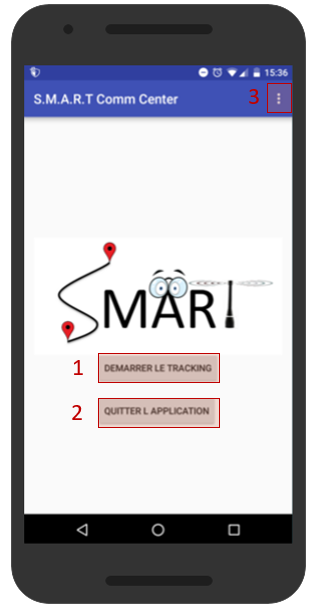
\includegraphics[width=.4\textwidth]{Ecran_accueil}
 		 \caption{Écran d'accueil}
 	 \label{fig:Ecran_accueil}
	\end{figure}
	~\\
	
	 La fenêtre ou écran d'accueil ne comprends qu'un bouton permettant de lancer l'activité de localisation et donc le client web et un bouton pour quitter l'application, accompagnés du logo du projet. Un menu déroulant a été implémenté de façon a pouvoir accéder aux paramètres.
	
	\begin{figure}[!h]
  	\centering
 	 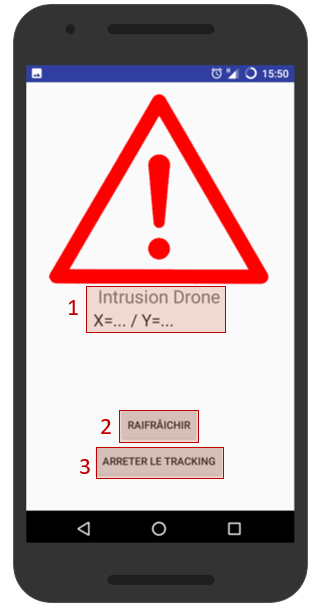
\includegraphics[width=.4\textwidth]{Ecran_loc}
 		 \caption{Écran de localisation}
 	 \label{fig:Ecran_loc}
	\end{figure}
	~\\
	
	 La fenêtre ou écran de localisation est un peu plus complexe. Pour l'utilisateur, les trois éléments clef de l'interface sont : les informations concernant l'état du système, le bouton "rafraîchir" et le bouton "retour". Un indicateur visuel est aussi présent en cas de détection d'intrusion.

	\begin{figure}[!h]
  	\centering
 	 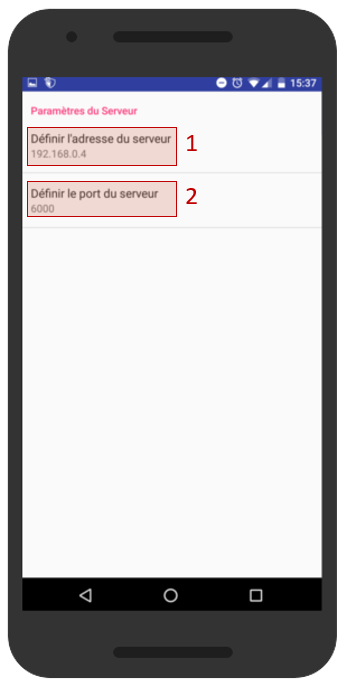
\includegraphics[width=.4\textwidth]{Ecran_set}
 		 \caption{Écran de localisation}
 	 \label{fig:Ecran_set}
	\end{figure}
	~\\	
	
	 La fenêtre de paramètres permet de modifier les paramètres de connexion du client comme l'adresse et le port du serveur visé.
		
	
\subsubsection{Détails concernant la fenêtre de localisation}

	La fenêtre de localisation comporte une particularité essentielle. En effet, en même temps que celle ci s'affiche, le client web est lancé en arrière plan grâce à une "AsynchTask" (Tâche asynchrone). L'intérêt d'un tel mode de fonctionnement présente l'avantage de ne pas avoir a créer de "Thread" (Fil d'exécution) supplémentaire et de découpler le serveur de l'affichage. Ainsi, en cas d'erreur de connexion ou de problème irrécupérable, l'interface continue de répondre et permet à l'utilisateur de relancer la connexion. Le système Android gèrera en parallèle l'affichage et le serveur, le fonctionnement des AsyncTask permet de s'assurer que tant que la fenêtre de l'application est visible par l'utilisateur le client fonctionnera en arrière plan.
	
	 

	

%%% Local Variables: 
%%% mode: latex
%%% TeX-master: "../rapport"
%%% End: 